\documentclass[english,hidelinks,pdftex, 11 pt, class=report,crop=false]{standalone}
\usepackage[T1]{fontenc}
\usepackage[utf8]{luainputenc}
\usepackage{lmodern} % load a font with all the characters
\usepackage{geometry}
\geometry{verbose,paperwidth=16.1 cm, paperheight=24 cm, inner=2.3cm, outer=1.8 cm, bmargin=2cm, tmargin=1.8cm}
\setlength{\parindent}{0bp}
\usepackage{import}
\usepackage[subpreambles=false]{standalone}
\usepackage{amsmath}
\usepackage{amssymb}
\usepackage{esint}
\usepackage{babel}
\usepackage{tabu}
\makeatother
\makeatletter

\usepackage{titlesec}
\usepackage{ragged2e}
\RaggedRight
\raggedbottom
\frenchspacing

% Norwegian names of figures, chapters, parts and content
\addto\captionsenglish{\renewcommand{\figurename}{Figur}}
\makeatletter
\addto\captionsenglish{\renewcommand{\chaptername}{Kapittel}}
\addto\captionsenglish{\renewcommand{\partname}{Del}}

\addto\captionsenglish{\renewcommand{\contentsname}{Innhald}}

\usepackage{graphicx}
\usepackage{float}
\usepackage{subfig}
\usepackage{placeins}
\usepackage{cancel}
\usepackage{framed}
\usepackage{wrapfig}
\usepackage[subfigure]{tocloft}
\usepackage[font=footnotesize,labelfont=sl]{caption} % Figure caption
\usepackage{bm}
\usepackage[dvipsnames, table]{xcolor}
\definecolor{shadecolor}{rgb}{0.105469, 0.613281, 1}
\colorlet{shadecolor}{Emerald!15} 
\usepackage{icomma}
\makeatother
\usepackage[many]{tcolorbox}
\usepackage{multicol}
\usepackage{stackengine}

% For tabular
\usepackage{array}
\usepackage{multirow}
\usepackage{longtable} %breakable table

% Ligningsreferanser
\usepackage{mathtools}
\mathtoolsset{showonlyrefs}

% index
\usepackage{imakeidx}
\makeindex[title=Indeks]

%Footnote:
\usepackage[bottom, hang, flushmargin]{footmisc}
\usepackage{perpage} 
\MakePerPage{footnote}
\addtolength{\footnotesep}{2mm}
\renewcommand{\thefootnote}{\arabic{footnote}}
\renewcommand\footnoterule{\rule{\linewidth}{0.4pt}}
\renewcommand{\thempfootnote}{\arabic{mpfootnote}}

%colors
\definecolor{c1}{cmyk}{0,0.5,1,0}
\definecolor{c2}{cmyk}{1,0.25,1,0}
\definecolor{n3}{cmyk}{1,0.,1,0}
\definecolor{neg}{cmyk}{1,0.,0.,0}

% Lister med bokstavar
\usepackage[inline]{enumitem}

\newcounter{rg}
\numberwithin{rg}{chapter}
\newcommand{\reg}[2][]{\begin{tcolorbox}[boxrule=0.3 mm,arc=0mm,colback=blue!3] {\refstepcounter{rg}\phantomsection \large \textbf{\therg \;#1} \vspace{5 pt}}\newline #2  \end{tcolorbox}\vspace{-5pt}}

\newcommand\alg[1]{\begin{align} #1 \end{align}}

\newcommand\eks[2][]{\begin{tcolorbox}[boxrule=0.3 mm,arc=0mm,enhanced jigsaw,breakable,colback=green!3] {\large \textbf{Eksempel #1} \vspace{5 pt}\\} #2 \end{tcolorbox}\vspace{-5pt} }

\newcommand{\st}[1]{\begin{tcolorbox}[boxrule=0.0 mm,arc=0mm,enhanced jigsaw,breakable,colback=yellow!12]{ #1} \end{tcolorbox}}

\newcommand{\spr}[1]{\begin{tcolorbox}[boxrule=0.3 mm,arc=0mm,enhanced jigsaw,breakable,colback=yellow!7] {\large \textbf{Språkboksen} \vspace{5 pt}\\} #1 \end{tcolorbox}\vspace{-5pt} }

\newcommand{\sym}[1]{\colorbox{blue!15}{#1}}

\newcommand{\info}[2]{\begin{tcolorbox}[boxrule=0.3 mm,arc=0mm,enhanced jigsaw,breakable,colback=cyan!6] {\large \textbf{#1} \vspace{5 pt}\\} #2 \end{tcolorbox}\vspace{-5pt} }

\newcommand\algv[1]{\vspace{-11 pt}\begin{align*} #1 \end{align*}}

\newcommand{\regv}{\vspace{5pt}}
\newcommand{\mer}{\textsl{Merk}: }
\newcommand\vsk{\vspace{11pt}}
\newcommand\vs{\vspace{-11pt}}
\newcommand\vsb{\vspace{-16pt}}
\newcommand\sv{\vsk \textbf{Svar:} \vspace{4 pt}\\}
\newcommand\br{\\[5 pt]}
\newcommand{\asym}[1]{../fig/#1}
\newcommand\algvv[1]{\vs\vs\begin{align*} #1 \end{align*}}
\newcommand{\y}[1]{$ {#1} $}
\newcommand{\os}{\\[5 pt]}
\newcommand{\prbxl}[2]{
\parbox[l][][l]{#1\linewidth}{#2
	}}
\newcommand{\prbxr}[2]{\parbox[r][][l]{#1\linewidth}{
		\setlength{\abovedisplayskip}{5pt}
		\setlength{\belowdisplayskip}{5pt}	
		\setlength{\abovedisplayshortskip}{0pt}
		\setlength{\belowdisplayshortskip}{0pt} 
		\begin{shaded}
			\footnotesize	#2 \end{shaded}}}

\renewcommand{\cfttoctitlefont}{\Large\bfseries}
\setlength{\cftaftertoctitleskip}{0 pt}
\setlength{\cftbeforetoctitleskip}{0 pt}

\newcommand{\bs}{\\[3pt]}
\newcommand{\vn}{\\[6pt]}
\newcommand{\fig}[1]{\begin{figure}
		\centering
		\includegraphics[]{\asym{#1}}
\end{figure}}


\newcommand{\sectionbreak}{\clearpage} % New page on each section

% Equation comments
\newcommand{\cm}[1]{\llap{\color{blue} #1}}

\newcommand\fork[2]{\begin{tcolorbox}[boxrule=0.3 mm,arc=0mm,enhanced jigsaw,breakable,colback=yellow!7] {\large \textbf{#1 (forklaring)} \vspace{5 pt}\\} #2 \end{tcolorbox}\vspace{-5pt} }




%colors
\newcommand{\colr}[1]{{\color{red} #1}}
\newcommand{\colb}[1]{{\color{blue} #1}}
\newcommand{\colo}[1]{{\color{orange} #1}}
\newcommand{\colc}[1]{{\color{cyan} #1}}
\definecolor{projectgreen}{cmyk}{100,0,100,0}
\newcommand{\colg}[1]{{\color{projectgreen} #1}}

%%% SECTION HEADLINES %%%

% Our numbers
\newcommand{\likteikn}{Likskapsteiknet}
\newcommand{\talsifverd}{Tal, siffer og verdi}
\newcommand{\koordsys}{Koordinatsystem}

% Calculations
\newcommand{\adi}{Addisjon}
\newcommand{\sub}{Subtraksjon}
\newcommand{\gong}{Multiplikasjon (Gonging)}
\newcommand{\del}{Divisjon (deling)}

%Factorization and order of operations
\newcommand{\fak}{Faktorisering}
\newcommand{\rrek}{Reknerekkefølge}

%Fractions
\newcommand{\brgrpr}{Introduksjon}
\newcommand{\brvu}{Verdi, utviding og forkorting av brøk}
\newcommand{\bradsub}{Addisjon og subtraksjon}
\newcommand{\brgngheil}{Brøk gonga med heiltal}
\newcommand{\brdelheil}{Brøk delt med heiltal}
\newcommand{\brgngbr}{Brøk gonga med brøk}
\newcommand{\brkans}{Kansellering av faktorar}
\newcommand{\brdelmbr}{Deling med brøk}
\newcommand{\Rasjtal}{Rasjonale tal}

%Negative numbers
\newcommand{\negintro}{Introduksjon}
\newcommand{\negrekn}{Dei fire rekneartane med negative tal}
\newcommand{\negmeng}{Negative tal som mengde}

% Geometry 1
\newcommand{\omgr}{Omgrep}
\newcommand{\eignsk}{Eigenskapar for trekantar og firkantar}
\newcommand{\omkr}{Omkrins}
\newcommand{\area}{Areal}

%Algebra 
\newcommand{\algintro}{Introduksjon}
\newcommand{\pot}{Potensar}
\newcommand{\irrasj}{Irrasjonale tal}

%Equations
\newcommand{\ligintro}{Introduksjon}
\newcommand{\liglos}{Løysing ved dei fire rekneartane}
\newcommand{\ligloso}{Løysingsmetodane oppsummert}

%Functions
\newcommand{\fintro}{Introduksjon}
\newcommand{\lingraf}{Lineære funksjonar og grafar}

%Geometry 2
\newcommand{\geoform}{Formlar for areal og omkrins}
\newcommand{\kongogsim}{Kongruente og formlike trekantar}
\newcommand{\geofork}{Forklaringar}

% Names of rules
\newcommand{\gangdestihundre}{Å gange desimaltall med 10, 100 osv.}
\newcommand{\delmedtihundre}{Deling med 10, 100, 1\,000 osv.}
\newcommand{\ompref}{Omgjøring av prefikser}
\newcommand{\adkom}{Addisjon er kommutativ}
\newcommand{\gangkom}{Multiplikasjon er kommutativ}
\newcommand{\brdef}{Brøk som omskriving av delestykke}
\newcommand{\brtbr}{Brøk gonga med brøk}
\newcommand{\delmbr}{Brøk delt på brøk}
\newcommand{\gangpar}{Gonging med parentes (distributiv lov)}
\newcommand{\gangparsam}{Parantesar gonga saman}
\newcommand{\gangmnegto}{Gonging med negative tal I}
\newcommand{\gangmnegtre}{Gonging med negative tal II}
\newcommand{\konsttre}{Konstruksjon av trekantar}
\newcommand{\kongtre}{Kongruente trekantar}
\newcommand{\topv}{Toppvinklar}
\newcommand{\trisum}{Summen av vinklane i ein trekant}
\newcommand{\firsum}{Summen av vinklane i ein firkant}
\newcommand{\potgang}{Gonging med potensar}
\newcommand{\potdivpot}{Divisjon med potensar}
\newcommand{\potanull}{Spesialtilfellet \boldmath $a^0$}
\newcommand{\potneg}{Potens med negativ eksponent}
\newcommand{\potbr}{Brøk som grunntal}
\newcommand{\faktgr}{Faktorar som grunntal}
\newcommand{\potsomgrunn}{Potens som grunntal}
\newcommand{\arsirk}{Arealet til ein sirkel}
\newcommand{\artrap}{Arealet til eit trapes}
\newcommand{\arpar}{Arealet til eit parallellogram}
\newcommand{\pyt}{Pytagoras' setning}
\newcommand{\forform}{Forhold i formlike trekantar}
\newcommand{\vilkform}{Vilkår i formlike trekantar}
\newcommand{\omkrsirk}{Omkrinsen til ein sirkel (og $ \bm \pi $)}
\newcommand{\artri}{Arealet til ein trekant}
\newcommand{\arrekt}{Arealet til eit rektangel}
\newcommand{\liknflyt}{Flytting av ledd over likskapsteiknet}
\newcommand{\funklin}{Lineære funksjonar}

%Opg
\newcommand{\abc}[1]{
	\begin{enumerate}[label=\alph*),leftmargin=18pt]
		#1
	\end{enumerate}
}
\newcommand{\abcs}[2]{
	\begin{enumerate}[label=\alph*),start=#1,leftmargin=18pt]
		#2
	\end{enumerate}
}
\newcommand{\abcn}[1]{
	\begin{enumerate}[label=\arabic*),leftmargin=18pt]
		#1
	\end{enumerate}
}
\newcommand{\abch}[1]{
	\hspace{-2pt}	\begin{enumerate*}[label=\alph*), itemjoin=\hspace{1cm}]
		#1
	\end{enumerate*}
}
\newcommand{\abchs}[2]{
	\hspace{-2pt}	\begin{enumerate*}[label=\alph*), itemjoin=\hspace{1cm}, start=#1]
		#2
	\end{enumerate*}
}

\newcommand{\opgt}{\phantomsection \addcontentsline{toc}{section}{Oppgaver} \section*{Oppgaver for kapittel \thechapter}\vs \setcounter{section}{1}}
\newcounter{opg}
\numberwithin{opg}{section}
\newcommand{\op}[1]{\vspace{15pt} \refstepcounter{opg}\large \textbf{\color{blue}\theopg} \vspace{2 pt} \label{#1} \\}
\newcommand{\ekspop}[1]{\vsk\textbf{Gruble \thechapter.#1}\vspace{2 pt} \\}
\newcommand{\nes}{\stepcounter{section}
	\setcounter{opg}{0}}
\newcommand{\opr}[1]{\vspace{3pt}\textbf{\ref{#1}}}
\newcommand{\oeks}[1]{\begin{tcolorbox}[boxrule=0.3 mm,arc=0mm,colback=white]
		\textit{Eksempel: } #1	  
\end{tcolorbox}}
\newcommand\opgeks[2][]{\begin{tcolorbox}[boxrule=0.1 mm,arc=0mm,enhanced jigsaw,breakable,colback=white] {\footnotesize \textbf{Eksempel #1} \\} \footnotesize #2 \end{tcolorbox}\vspace{-5pt} }

%License
\newcommand{\lic}{\textit{Matematikken sine byggesteinar by Sindre Sogge Heggen is licensed under CC BY-NC-SA 4.0. To view a copy of this license, visit\\ 
		\net{http://creativecommons.org/licenses/by-nc-sa/4.0/}{http://creativecommons.org/licenses/by-nc-sa/4.0/}}}

%referances
\newcommand{\net}[2]{{\color{blue}\href{#1}{#2}}}
\newcommand{\hrs}[2]{\hyperref[#1]{\color{blue}\textsl{#2 \ref*{#1}}}}
\newcommand{\rref}[1]{\hrs{#1}{Regel}}
\newcommand{\refkap}[1]{\hrs{#1}{Kapittel}}
\newcommand{\refsec}[1]{\hrs{#1}{Seksjon}}

\usepackage{datetime2}

\usepackage[]{hyperref}


\begin{document}
\section{Addisjon}

\subsubsection{Oppstilling}
Denne metoden baserer seg på plassverdisystemet, der ein trinnvis rekner ut summen av einarane, tiarane, hundrerane, o.l.

\begin{center}
	\parbox{0.3\linewidth}{
\eks[1]{
	\begin{figure}
		\centering
		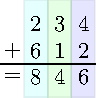
\includegraphics[]{rekfig/plus1}
	\end{figure}
}
}\qquad
\parbox{0.3\linewidth}{
\eks[2]{
	\begin{figure}
		\centering
		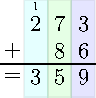
\includegraphics[]{rekfig/plus2}
	\end{figure}
}
}\\[12pt]
\parbox{0.3\linewidth}{
\eks[3]{
	\begin{figure}
		\centering
		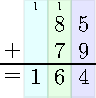
\includegraphics[]{rekfig/plus3}
	\end{figure}
}}\qquad
\parbox{0.3\linewidth}{
\eks[4]{
	\begin{figure}
		\centering
		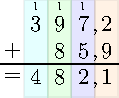
\includegraphics[]{rekfig/plus4}
	\end{figure}
}}
\end{center}
\fork{Eksempel 1}{
\begin{figure}
	\centering
	\subfloat[]{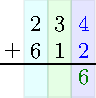
\includegraphics{rekfig/plus1a}}\qquad
	\subfloat[]{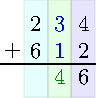
\includegraphics{rekfig/plus1b}}\qquad
	\subfloat[]{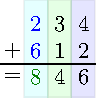
\includegraphics{rekfig/plus1c}}
\end{figure}

\begin{enumerate}[label=\alph*)]
	\item Vi legg saman einarane: $ 4+2=6 $
	\item Vi legg saman tiarane: $ 3+1=4 $
	\item Vi legg saman hundra: $ 2+6=8 $
\end{enumerate}
} \newpage
\fork{Eksempel 2}{
	\begin{figure}
		\centering
		\subfloat[]{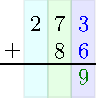
\includegraphics{rekfig/plus2a}}\qquad
		\subfloat[]{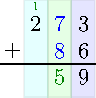
\includegraphics{rekfig/plus2b}}\qquad
		\subfloat[]{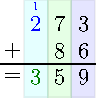
\includegraphics{rekfig/plus2c}}
	\end{figure}
	
	\begin{enumerate}[label=\alph*)]
		\item Vi legg saman einarane: $ 3+6=9 $
		\item Vi legg saman tiarane: $ {7+8=15} $. Sidan 10 tiarar er det same som 100, legg vi til 1 på hundreplassen, og skriv opp dei resterande 5 tiarane på tiarplassen.
		\item Vi legg saman hundra: $ 1+2=3 $.
	\end{enumerate}
} \vsk

\spr{
Det å skrive 1 på neste sifferplass kallast ''å skrive 1 i mente''.
}
\subsubsection{Tabellmetoden}
Denne metoden tar utgangspunkt i det éine leddet, og summerer fram til det andre leddet er nådd. Det som i starten kan vere litt rart med denne metoden, er at du sjølv velg fritt kva tall du skal legge til, så lenge du når det andre leddet til slutt.
\begin{center}
	\parbox{0.3\linewidth}{
		\eks[1]{
			$ \colb{273}+\colc{86} = \colo{359} $ \vsk
			
			\begin{tabular}{r|r|r}
				&&\colb{273} \\ \hline
				6 & 6 & 279 \\
				30& 36 & 309 \\
				50& \colc{86} & \colo{359}
			\end{tabular}
		}
	} \qquad
	\parbox{0.3\linewidth}{
		\eks[2]{
			$ \colb{85}+\colc{79}=\colo{164} $  \vsk
			
			\begin{tabular}{r|r|r}
				& & \colb{85} \\ \hline 
				5 & 5 & 90 \\
				10 & 15 &100 \\
				64 & \colc{79} & \colo{164} \\
			\end{tabular} \vsk
		}
	}
\end{center}
\newpage
\fork{Eksempel 1}{
\begin{figure}
	\centering
\subfloat[]{
\begin{tabular}{r|r|r}
	&&\colb{273} \\ \hline
	 &  &  \\
	\phantom{30}& \phantom{36} &  \\
	&  & 
\end{tabular}
} \qquad
\subfloat[]{
	\begin{tabular}{r|r|r}
		&&\colb{273} \\ \hline
		6& 6 & 279 \\
		\phantom{30}& \phantom{36} &  \\
		&  & 
	\end{tabular}
}\vsk 

\subfloat[]{
	\begin{tabular}{r|r|r}
		&&\colb{273} \\ \hline
		6& 6 & 279 \\
		30& 36 & 309  \\
		&  & 
	\end{tabular}
}
\qquad
\subfloat[]{
	\begin{tabular}{r|r|r}
		&&\colb{273} \\ \hline
		6& 6 & 279 \\
		30& 36 & 309  \\
		50& \colc{86} & \colo{359}
	\end{tabular}
}
\end{figure}
\begin{enumerate}[label=(\alph*)]
\item Vi startar med det leddet vi sjølv ønsker, ofte er det lurt å starte med det største leddet.
\item Vi legg til $ 6 $. Da har vi totalt lagt til $ 6 $, og vidare er $ {273+6=279} $.
\item Vi legg til 30. Da har vi så totalt lagt til 36, og vidare er $ 279+30=309 $.
\item Vi legg til 50. Da har vi totalt lagt til 86, altså har vi nådd det andre leddet, og vidare er $ 309+50=359 $.
\end{enumerate}
} \vsk

\info{Oppstilling versus tabellmetoden}{
	Ved første augekast kan kanskje tabellmetoden sjå ut som ein innvikla måte å rekne addisjon på samanlikna med oppstilling, men med øving vil mange oppdage at tabellmetoden betrer evnen til hoderekning.   
}

\section{Subtraksjon}
\subsubsection{Oppstilling}
Subtraksjon med oppstilling baserer seg på plassverdisystemet, der ein trinnvis rekner differansen mellom einarane, tiarane, hundra, o.l. Metoden tar også utgangspunkt i eit mengdeperspektiv, og tillet derfor ikkje differansar med negativ verdi (sjå forklaringa til \textsl{Eksempel 2}).
\begin{center}
	\parbox{0.3\linewidth}{
\eks[1]{
	\begin{figure}
		\centering
		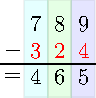
\includegraphics[]{rekfig/min1}
	\end{figure}
}} \qquad
\parbox{0.3\linewidth}{
\eks[2]{
	\begin{figure}
		\centering
		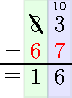
\includegraphics[]{rekfig/min2}
	\end{figure}
}} \\[12pt]
\parbox{0.3\linewidth}{
\eks[3]{
	\begin{figure}
		\centering
		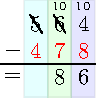
\includegraphics[]{rekfig/min3}
	\end{figure}
}}\qquad
\parbox{0.3\linewidth}{
\eks[4]{
	\begin{figure}
		\centering
		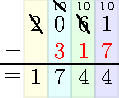
\includegraphics[]{rekfig/min4}
	\end{figure}
}}

\end{center}
\fork{Eksempel 1}{ \vs
\begin{figure}
	\centering
	\subfloat[]{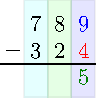
\includegraphics{rekfig/min1a}}\qquad
	\subfloat[]{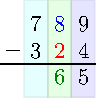
\includegraphics{rekfig/min1b}}\qquad
	\subfloat[]{
\includegraphics{rekfig/min1c}}
\end{figure}

\begin{enumerate}[label=(\alph*)]
	\item Vi finn differansen mellom einarane: $ {9-4=5} $
	\item Vi finn differansen mellom tiarane: $ {8-2=6} $. 
	\item Vi finn differansen mellom hundra: $ {7-3=4} $.
\end{enumerate}
}
\newpage
\fork{Eksempel 2}{ \vs
	\begin{figure}
		\centering
		\subfloat[]{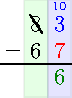
\includegraphics{rekfig/min2a}}\qquad
		\subfloat[]{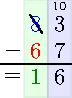
\includegraphics{rekfig/min2b}}
	\end{figure}
	
	\begin{enumerate}[label=(\alph*)]
		\item Vi merker oss at 7 er større enn 3, derfor tar vi 1 tiar frå dei 8 på tiarplassen. Dette markerer vi ved å sette ein strek over 8. Så finn vi differansen mellom einarane: $ {13-7=6} $
		\item Sidan vi tok 1 frå dei 8 tiarane, er der no berre 7 tiarar. Vi finn differansen mellom tiarane: $ {7-6=1} $.
	\end{enumerate}
}
\subsubsection{Tabellmetoden}
Tabellmetoden for subtraksjon tek utgangspunkt i at subtraksjon er ein omvend operasjon av addisjon. For eksempel, svaret på spørsmålet ''Kva er $ 789-324 $?'' er det same som svaret på spørsmålet ''Kor mykje må eg legge til på 324 for å få 789?''. Med tabellmetoden følg du ingen spesiell regel underveis, men velg sjølv talla du meiner passar best for å nå målet.\\
\begin{center}
\parbox{0.35\linewidth}{
\eks[1]{
$ \colb{789}-\colr{324}=\colc{465} $	 \vsk

\begin{tabular}{r|r}
	& \colr{324} \\ \hline
	6&330 \\
	70&400 \\
	389&\colb{789} \\ \hline
	\colc{465}
\end{tabular}
}} \qquad
\parbox{0.35\linewidth}{
	\eks[2]{
		$ \colb{83}-\colr{67}=\colc{16} $	 \vsk
		
		\begin{tabular}{r|r}
			& \colr{67} \\ \hline
			3&70 \\
			13&\colb{83} \\ \hline
			\colc{16}
		\end{tabular} \vspace{14pt}
}} \\[12pt]
\parbox{0.35\linewidth}{
	\eks[3]{
		$ 564-478=86 $\vsk
		
		\begin{tabular}{r|r}
			& 478 \\ \hline
			2&480 \\
			20&500 \\ 
			64&564\\ \hline
			86
		\end{tabular}
}} \qquad 
\parbox{0.4\linewidth}{
	\eks[4]{
		$ {206,1-31,7=174,4} $\vsk
		
		\begin{tabular}{r|r}
			& 31,7 \\ \hline
			0,3& 32\phantom{,0} \\
			70\phantom{,0}&102\phantom{,0} \\ 
			104,1&206,1\\ \hline
			174,4
		\end{tabular}
}}
\end{center}
\fork{Eksempel 1}{
	\[ \colb{789}-\colr{324}=\colo{465} \]
\begin{figure}
	\centering
	\subfloat[]{
	\begin{tabular}{r|r}
		& \colr{324} \\ \hline
		& \\
		& \\
		& \\ \hline
		&
	\end{tabular}	
} \qquad
	\subfloat[]{
	\begin{tabular}{r|r}
		& \colb{324} \\ \hline
	   \colb{6}& \colc{330}\\
		& \\
		& \\ \hline
		&
	\end{tabular}
}\qquad
	\subfloat[]{
	\begin{tabular}{r|r}
		& 324 \\ \hline
		6& \colb{330}\\
		\colb{70}& \colc{400} \\
		& \\ \hline
		&
	\end{tabular}	
}  \\[12pt]
\subfloat[]{
	\begin{tabular}{r|r}
		& 324 \\ \hline
		6& 330\\
		70& \colb{400} \\
		\colb{389}& \colc{789}\\ \hline
		&
	\end{tabular}	
}\qquad
\subfloat[]{
	\begin{tabular}{r|r}
		& 324 \\ \hline
		\colb{6}& 330\\
		\colb{70}& 400 \\
		\colb{389}& 789\\ \hline
		\colo{465}&
	\end{tabular}	
}
\end{figure}
\begin{enumerate}[label=(\alph*)]
	\item Vi startar med 324.
	\item Vi legg til 6, og får $ {324+6=330} $
	\item Vi legg til 70, og får $ {70+330=400} $
	\item Vi legg til 389, og får $ {389+400=789} $. Da er vi framme på 789.
	\item Vi summerer tala vi har lagt til:  $ {6+70+389=465} $
\end{enumerate}
}
\section{Ganging} \label{rekGanging}
\subsubsection{Ganging med 10, 100, 1\,000 osv.}
\reg[Å gonge heiltal med 10, 100 osv. \label{gangheiltalmed10100}]{
	\vs
	\begin{itemize}
		\item Når ein gongar eit heiltal med 10, får ein svaret ved å legge til sifferet 0 bak heiltalet.
		\item Når ein gongar eit heiltal med 100, får ein svaret ved å legge til sifra 00 bak heiltalet.
		\item Det same mønsteret gjelder for talla 1\,000, 10\,000 osv.
	\end{itemize}
}
\eks[1]{\vsb \vsb
	\alg{
		6\cdot \colb{10} &= 6\colb{0}\vn
		79\cdot \colb{10} &= 79\colb{0} \vn
		802\cdot\colb{10}&=802\colb{0}
	}
}
\eks[2]{ \vsb \vsb
\alg{ 
6\cdot\colb{100} &= 6\colb{00} \vn
79\cdot\colb{100} &= 7\,9\colb{00} \vn
802\cdot\colb{100} &=80\,2\colb{00}
}
}
\eks[3]{ \vsb \vsb
\alg{ 
	6\cdot\colb{1\,000} &= 6\,\colb{000} \vn
	79\cdot\colb{10\,000} &= 79\colb{0\,000} \vn
	802\cdot\colb{100\,000} &=80\,2\colb{00\,000}
}
}
\newpage
\reg[Å gonge desimaltal med 10, 100 osv. \label{gangdesmed10100}]{
	\vs
	\begin{itemize}
		\item Når ein gongar  eit  desimaltal med 10, får ein svaret ved å flytte komma en plass til høgre.
		\item Når ein gongar eit heiltal med 100, får ein svaret ved å flytte komma to plasser til høgre.
		\item Det same mønsteret gjelder for tallene 1\,000, 10\,000 osv.
	\end{itemize}
}
\eks[1]{\vsb \vsb
	\alg{
		7\colr{,}9\cdot 10 &= 79\colr{,}=79 \vn
		38\colr{,}02\cdot10&=380\colr{,}2 \vn
		0\colr{,}57\cdot 10 &=05\colr{,}7=5\colr{,}7 \vn
		0\colr{,}194\cdot 10&= 01\colr{,}94=1\colr{,}94
	}
}
\eks[2]{ \vsb \vsb
	\alg{
		7\colr{,}9\cdot 100 &= 790\colr{,}=790 \vn
		38\colr{,}02\cdot100&=3802\colr{,}=3\,802 \vn
		0\colr{,}57\cdot 100 &=057\colr{,}=57 \vn
		0\colr{,}194\cdot 100&= 019\colr{,}4=19\colr{,}4
	}
}
\eks[3]{ \vsb \vsb
	\alg{
	7\colr{,}9\cdot 1\,000 &= 7900\colr{,}=7\,900 \vn
	38\colr{,}02\cdot10\,000&=38020\colr{,}=38\,020 \vn
	0\colr{,}57\cdot 100\,000 &=05\colr{,}7=57000\colr{,}=57\,000
}
}
\info{Merk}{
\rref{gangheiltalmed10100} er berre  eit  spesialtilfelle av \rref{gangdesmed10100}. For eksempel, å bruke \rref{gangheiltalmed10100} på reknestykket $ {7\cdot 10} $ gir same resultat som å bruke \rref{gangdesmed10100} på reknestykket $ {7,0\cdot 10} $. 
}
\newpage
\fork{Å gonge tall med 10, 100 osv.}{
Titalsystemet baserer seg på grupper av ti, hundre, tusen osv., og tidelar, hundredelar og tusendelar osv. (sjå \rref{titalsys}). Når ein gongar  eit  tall med 10, vil alle einarane i talet bli til tiarar, alle tiarar bli til hundra osv. Kvart siffer forskyvast altså éin plass mot venstre. Tilsvarende forskyvast kvart siffer to plassar mot venstre når ein gongar med 100, tre plassar når ein gongar med 1\,000 osv.
}
\subsubsection{Utvida form}
Gonging på utvida form bruker vi for å rekne multiplikasjon mellom fleirsifra tall. Metoden baserer seg på distributiv lov (sjå \rref{gangpar}). \regv
\eks[1]{ \vs
\begin{figure}
	\centering
	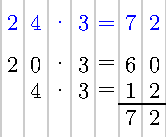
\includegraphics[]{rekfig/gang1}
\end{figure}
}
\eks[2]{ \vs
\begin{figure}
	\centering
	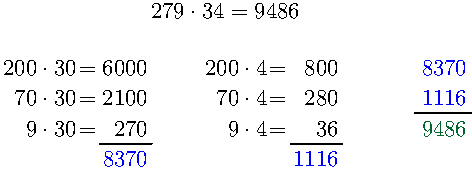
\includegraphics[]{rekfig/gfleirsif}
\end{figure}
}
\fork{Eksempel 1}{
24 kan skrivast som $ 20+4 $, altså er
\[ 24\cdot3 =(20+4)\cdot3 \]
Vidare er 
\algv{
(20+4)\cdot 3 &=20\cdot 3 + 4\cdot 3 \\
&= 60+12 \\
&= 72
}
}
\newpage
\fork{Eksempel 2}{
Vi har at
\alg{
279&=200+70+9 \\
34 &=30+4 	
}
Altså er
\alg{
279\cdot34&= (200+70+9)\cdot (30+4) 
}
Vidare er 
{
\footnotesize
\alg{
(200+70+9)\cdot (30+4) &=200\cdot 30+70\cdot30+9\cdot30+200\cdot4+70\cdot4+9\cdot4
\\
&=9486}
} \vs
}
\subsubsection{Kompaktmetoden}
Kompaktmetoden bygger på dei same prinsippa som gonging på utvida form, men har ein skrivemåte som gjer utrekninga kortare. \regv

\eks[1]{
	\begin{figure}
		\centering
		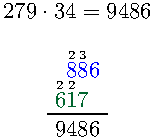
\includegraphics[]{rekfig/gfleirsifa}
	\end{figure}
}
\newpage
\fork{Eksempel 1}{
Vi startar med å gonge sifra i 279 enkeltvis med 4:
\begin{itemize}
	\item $ 9\cdot 6=36 $, da skriv vi 6 på einarplassen og 3 i mente.
	\item $ 7\cdot4 =28$, da skriv vi 8 på tiarplassen og 2 i mente.
	\item $ 2\cdot 4=8 $, da skriv vi 8 på hundrerplassen.
\end{itemize}
Så gongar vi sifra i 279 enkeltvis med 30. Dette kan forenklast til å gonge med 3, så lenge vi plasserer sifra én plass forskyvde til venstre i forhold til da vi gonga med 4:
\begin{itemize}
	\item $ 9\cdot 3=27 $, da skriv vi 7 på tiarplassen og 2 i mente. 
	\item $ 7\cdot3=21 $, da skriv vi 1 på hundrerplassen og 2 i mente.
	\item $ 2\cdot3=6 $, da skriv vi 6 på tusenplassen.
\end{itemize} 
}
\section{Divisjon} \label{rekDivisjon}
\subsubsection{\delmedtihundre}
\reg[Deling med 10, 100, 1\,000 osv. \label{deledesmed10100}]{ \vs
\begin{itemize}
	\item Når ein deler  eit  desimaltal med 10, får ein svaret ved å flytte komma en plass til venstre.
	\item Når ein deler  eit  desimaltal med 10, får ein svaret ved å flytte komma to plasser til venstre.
	\item Det same mønsteret gjelder for tallene 1\,000, 10\,000 osv.
\end{itemize}
}
\eks[1]{ \vsb \vsb
	\alg{
200:10&=200\colr{,}0:10 \\&=20\colr{,}00\\&=20	\vn
45:10&=45\colr{,}0:10 \\&= 4\colr{,}50 \\&=4\colr{,}5
}
}
\eks[2]{ \vsb \vsb
	\alg{
		200:100&=200\colr{,}0:100 \\&=2\colr{,}000\\&=2	\vn
		45:100&=45\colr{,}0:100 \\&= 0\colr{,}450 \\&=0\colr{,}45
	}
}
\newpage
\eks[3]{ \vsb \vsb
\alg{
143\colr{,}7 :10 &= 14\colr{,}37 \vn
143\colr{,}7 :100 &= 1\colr{,}437 \vn
143\colr{,}7 :1\,000 &= 0\colr{,}1437 \vn
93\colr{,}6:10 &= 9\colr{,}36 \vn
93\colr{,}6:100 &= 0\colr{,}936 \vn
93\colr{,}6:1\,000 &= 0\colr{,}0936
}
}
\fork{Deling med 10, 100, 1\,000 osv.}{
Titalsystemet baserer seg på grupper av ti, hundre, tusen osv., og tideler, hundredeler og tusendeler osv (sjå \rref{titalsys}). Når ein deler  eit  tall med 10, vil alle einare i tallet bli til tidelar, alle tiarar bli til einarar osv. Kvart siffer forskyvast altså éin plass mot høgre. Tilsvarande forskyvast kvart siffer to plassar mot høgre når ein deler med 100, tre plassar når ein deler med 1\,000 osv.
}

\subsubsection{Oppstilling}
Divisjon med oppstilling baserer seg på divisjon tolka som inndeling av mengder (sjå s.\pageref{Divisjon})

\begin{center}
	\parbox{0.3\linewidth}{
	\eks[1]{ \vsb
		\begin{figure}
			\centering
			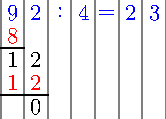
\includegraphics[]{rekfig/del1}
		\end{figure} \vspace{18pt}
	}
}\qquad
\parbox{0.45\linewidth}{
	\eks[1]{ \vspace{-5pt}
		\begin{figure}
			\centering
			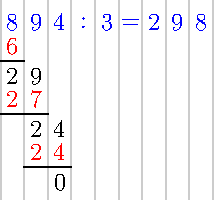
\includegraphics[]{rekfig/del2}
		\end{figure}
	}
}
\end{center}
\newpage
\subsubsection{Tabellmetoden}
Tabellmetoden baserer seg på divisjon som omvend operasjon av gonging. For eksempel er svaret på spørsmålet ''Kva er $ {76:4} $'' det same som svaret på spørsmålet ''Kva tal må eg gonge 4 med for å få 76?''. På same vis som for tabellmetoden ved subtraksjon er det opp til ein sjølv å velge passande tal for å nå målet.
\begin{center}
	\parbox{0.35\linewidth}{
		\eks[1]{
			$ \colg{76}:\colb{4}=\colo{19} $	 \vsk
			
			\begin{tabular}{r|r|r}
				$ \cdot\, \colb{4} $&\\ \hline
				10&40&40 \\
				9& 36 &\colg{76} \\ \hline
				\colo{19}&
			\end{tabular}
		\vspace{42pt}
	}} \qquad
\parbox{0.35\linewidth}{
	\eks[2]{
		$ \colg{894}:\colb{3}=\colo{298} $	 \vsk
		
		\begin{tabular}{r|r|r}
			$ \cdot\, \colb{3} $&\\ \hline
			200& 600 &600 \\
			60&120 &720 \\
			60&120 &840 \\
			10& 30&870 \\
			8&24 &\colg{894} \\ \hline
			\colo{298} &
		\end{tabular}
}} \vsk

\parbox{0.415\linewidth}{
	\eks[3]{		
		$ 894:3=298 $	 \vsk
		
		\begin{tabular}{r|r|r}
			$ \cdot\, 3 $&\\ \hline
			300& 900&900 \\
			$ -2 $& $ -6 $ &894 \\ \hline
			298&
		\end{tabular} \vsk
	
\footnotesize	
\mer same reknestykke som i \textsl{Eksempel 2}, men ei anna utrekning.
}
}
\end{center}

\section{Primtalsfaktorisering \label{primtalsfakt}}
\mer Primtala mellom 1-100 finn du på side \pageref{primtalfig}.


\begin{center}
		\parbox{0.35\linewidth}{
	\eks[1]{
		$ \colo{84}= \colb{2\cdot2\cdot3\cdot7}$	 \vsk
		
		\begin{tabular}{r|r|r}
			& $ : $&\\ \hline
			\colo{84}&\colb{2}&\colg{42} \\
			\colg{42}& \colb{2} &\colg{21} \\ 
			\colg{21}&\colb{3}&\colb{7}\\
			\hline
		\end{tabular}
}} \qquad
\parbox{0.35\linewidth}{
	\eks[2]{
		$ \colo{595}= \colb{5\cdot7\cdot17}$	 \vsk
		
		\begin{tabular}{r|r|r}
			& $ : $&\\ \hline
			\colo{595}& \colb{5} &\colg{119} \\ 
			\colg{119}&\colb{7}&\colb{17}\\
			\hline
		\end{tabular}
	\vspace{12pt}
}}
\end{center} 


\fork{Eksempel 1}{ \vs
\begin{figure}
	\centering
	\subfloat[]{
		\begin{tabular}{r|r|r}
			& $ : $&\\ \hline
			\colo{84}&\colb{2}&\colg{42} \\
			&& \\ 
			&&\\
			\hline
		\end{tabular}
	} \qquad
	\subfloat[]{
		\begin{tabular}{r|r|r}
			& $ : $&\\ \hline
			\colo{84}&\colb{2}&\colg{42} \\
			\colg{42}& \colb{2} &21 \\ 
			&&\\
			\hline
		\end{tabular}
	}\vsk 
	
	\subfloat[]{
		\begin{tabular}{r|r|r}
			& $ : $&\\ \hline
			\colo{84}&\colb{2}&42 \\
			42& \colb{2} &\colg{21} \\ 
			\colg{21}&\colb{3}&\colb{7}\\
			\hline
		\end{tabular}
	}
\end{figure}
\begin{enumerate}[label=(\alph*)]
\item Sidan 2 er det første primtallet, undersøker vi om 84 er deleleg med 2. Det er det, fordi $ 84:2=42 $.
\item Vi undersøker om også 42 er deleleg med 2. Det er det, fordi $ 42:2=21 $.
\item Vi undersøker om også 21 er deleleg med 2. Det er det ikkje, fordi $ {21:2=10,5} $. Derfor går vi over til neste primtall, som er 3. 21 er deleleg med 3 fordi $ 21:3=7 $.
\end{enumerate}
Sidan 7 er eit primtal, er vi komme i mål.
}
\newpage
\label{primtalfig}
\fig{primn100}
\end{document}

